\documentclass[a4paper,12pt,openright,twoside]{report}
%\usepackage[hmarginratio=3:2,vmarginratio=1:1]{geometry}
%\usepackage[top=2cm,bottom=4cm,left=1.5cm,right=3cm]{geometry}
\usepackage{amsmath}
\usepackage{subcaption}
\usepackage{emptypage}
\usepackage{subdepth}
\usepackage{amssymb}
\usepackage{mathrsfs}
\usepackage[sort&compress]{natbib}
\usepackage{graphics}
\usepackage{fancyhdr}
\usepackage{graphicx}
\usepackage{braket}
\usepackage{epigraph}
\usepackage{bm}
\usepackage{multirow}
\usepackage[LGRx,T1]{fontenc} % notice LGRx instead of LGR
\usepackage[utf8]{inputenc}   % utf8 is required
%\usepackage{textgreek}
\newcommand{\textgreek}[1]{\begingroup\fontencoding{LGR}\selectfont#1\endgroup}
\let\tmp\oddsidemargin
\let\oddsidemargin\evensidemargin
\let\evensidemargin\tmp
\reversemarginpar
\citestyle{nature}
\bibliographystyle{phjcp}
\linespread{1.2}

\newcommand*{\LargerCdot}{\raisebox{-0.25ex}{\scalebox{1.2}{$\cdot$}}}

\begin{document}
\cleardoublepage
\begin{titlepage}

\begin{center}
\linespread{1.3}
\textsc{\LARGE Approaching the Marangoni Effect through\\}
\textsc{\LARGE equilibrium molecular dynamics\\}
\vfill
\sc{H. G. A. Burton\\
Robinson College\\
Cambridge}

\vfill 


\includegraphics[width=0.3\textwidth]{Robinson_College_Crest.png}

\vfill 

\end{center}
\end{titlepage}

\cleardoublepage
%\newpage
\pagenumbering{roman}
\thispagestyle{empty}
\cleardoublepage
%\pagenumbering{roman}
\section*{Acknowledgements}
\addcontentsline{toc}{chapter}{Acknowledgements}

Acknowledgements go here.

\newpage

\cleardoublepage
\thispagestyle{plain}
\addcontentsline{toc}{section}{Abstract}
\begin{center}
%\linespread{1.3}   
\textsc{\Large Holomorphic Hartree--Fock Theory:\\ From Formulation to Application}

    \vspace{0.2cm}
    \normalsize{{\textsc{Hugh Graham Alexander Burton}}}
    
\vspace{0.2cm}
    \normalsize{\textbf{Abstract}}
\end{center}
ABSTRACT GOES HERE

%\begin{abstract}
%The abstract goes here.
%\end{abstract}
\newpage

\tableofcontents
\cleardoublepage
\listoffigures
\addcontentsline{toc}{chapter}{List of Figures}
\cleardoublepage
\listoftables
\addcontentsline{toc}{chapter}{List of Tables}


\newpage
\cleardoublepage
\pagenumbering{arabic}
\fancyhead{}
\rhead{\thepage}
\lhead{\leftmark}
\lfoot[]{}
\rfoot[]{}
\cfoot[]{}
\fancypagestyle{plain}{
    \fancyhf{} % clear all header and footer fields
    \fancyhead{} % except the right top corner
    \renewcommand{\headrulewidth}{0pt} % remove line between header and main text
}
\pagestyle{fancy}
%\renewcommand{\chaptermark}[1]{\markboth{#1}{}}
%\renewcommand{\chaptermark}[1]{\markboth{\MakeUppercase{\chaptername}\ \thechapter. \ #1}{}}
%\renewcommand{\chaptermark}[1]{\markboth{\MakeUppercase{\chaptername} #1}{}}
%\renewcommand{\chaptermark}[1]{
%    \markboth{\MakeUppercase{
%            \chaptername\ \thechapter.
%\ #1}}{}}
\renewcommand{\chaptermark}[1]{
\markboth{\MakeUppercase{#1}}{}}
\fancyhead[LO]{\leftmark}
\fancyhead[RE]{\leftmark}
\fancyhead[LE,RO]{\thepage}
    
\section{Introduction}
2015 saw the $160^{\mathrm{th}}$ anniversary of J. Thompson's first report\cite{JThompson} on the observation of flows occuring at a fluid--fluid interface as the result of a tangential chemical potential or temperature gradient.
This phenomenom was later termed the ``Marangoni Effet'' after it formed the basis of Carlo Marangoni's doctoral dissertation.\cite{Marangoni}
Since then temperature induced Marangoni flows, also known as thermocapillary flows, have been the subject of a number of studies and a macroscopic description has been developed through the works of Derjaguin\cite{SurfaceForces} and Levich\cite{Levich}, as summarised in the context of phoresis by Anderson\cite{Anderson}.

On the simplest level this effect can be described as a flow occuring due to a gradient in the surface--tension at the interface, with motion occuring from regions of low to regions of high surface--tenson.
However, this is not particulaly informative since the temperature dependence of surface--tension is itself known only through empirical studies.
Beyond a surface--tension based description, Derjaguin demonstrated that the flow can be calculated from the excess enthalpy of a fluid close to the interface, hence formulating a thermodynamic theory of thermocapillary motion.\cite{SurfaceForces}

The thermodynamic backbone upon which this theory is founded is reliant on knowledge of the macroscopic properties of the system.
In contrast, the flow itself is inherently a microscopic phenomenon acting in a localised way at the interfaces of bulk fluids. 
Such a localised effect cannot be faithfully described using a macroscopic thermodynamic description, instead it requires a microscopic theory formulated around the interpaticle interactions. 
No such theory currently exists, and there have been a very limited number of studies in this area.\cite{HolgerBoppHampe}
By studying the microscopic properties of a liqud--liquid interface, this report aims model the Maragnoni effect and investigate the link between these microscopic properties and the macroscopic fluid motion.

\subsection{Experimental studies}
Despite the lack of a microscopic theory, there has been substantial experimental research into the Marangoni effect.
Many of these studies have focussed on the more curious examples of Marangoni flows such as Thompson's ``tears of wine''\cite{JThompson,Venerus,Tadmor,Cazabat1995} and the ``coffee ring effect'',\cite{Sefian,HuLarson,Sefiane2014} whilst others have shown it is becoming ever more important in technological applications.
For example, Sternling and Scriven\cite{SternlingScriven} proposed Marangoni effects as the origin for interfacial turbelence and mass transport, yielding applications in fluid mixing and oil recovery,\cite{Aguilera2005,LyfordA,LyfordB} whilst Subramanian and Balasubramanian outline the importance of Marangoni forces for the motion of bubbles and droplets in reduced gravity environments.\cite{MotionOfBubblesAndDrops} 

In 1959, Young et al. produced a theoretical description of this motion of bubbles and droplets under the influence of a temperature gradient, a phenomena described as thermophoresis.\cite{Young1959}
They describe how the temperature gradient causes a higher surface--tension on the low temperature side of the droplet, resulting in a force pulling the surrounding fluid towards the low temperature region and a corresponding reaction force propelling the droplet towards the warmer fluid region (note the similarity to electrophoresis where there is no-net force within the droplet).
This force was measured experimentally by S. C. Hardy,\cite{Hardy1978} who used a temperature gradient to balance the Marangoni and buoyancy forces acting on a droplet within a fluid, thus holding the droplet stationary.
Later theoretical modelling by Kim and Subramanian suggested that the inclusion of surface--active substances could be used to prevent thermophoresis,\cite{KimSubramanianA,KimSubramanianB} a prediction that was later confirmed experimentally.\cite{BartonSubramanian,ChenStebe}

With the advances in space technology over the past half a century, thermophoresis and thermocapillary motion have become important mechanisms for fluid motion and mass transfer in low--gravity environments, where surface effects dominate over buoyancy driven motion.
The motion of bubbles and drops due to interfacial gradients is considered to be key for materials processing in space, enabling phase separation of binary mixtures and the potential to make uniform composite materials.\cite{BartonSubramanian}
Moreover, fluid transport in the absence of gravity is important for controlling fluid fuels aboard satellites, often carried for thrusters used to perform orbital adjustments.\cite{MotionOfBubblesAndDrops} 

\subsection{Striving for a microscopic description}
With so many potential applications, the search for a micrcoscpic description is becoming ever more significant and computer simulations are increasingly being used to understand this phenomenom.
Marangoni flows are inherently dynamic and must be studied using a time--dependent siumulation method such as Molecular Dynamics (henceforth MD).
To model the dynamic behaviour of an immiscible binary--mixture under the effect of a temperature gradient might initially appear trivial; simply create a temperature gradient for such a system and measure the expected flow velocity of the resulting particles.
This non-equilibirum approach is used by Hampe et al. in their study of the Marangoni effect.\cite{HolgerBoppHampe}
Despite their positive results, the method is complicated by the use of periodic boundary conditions (required to model a macroscopic fluid) that require each unit cell to have two temperature gradients such that the temperature is also periodic.
Any flow due to this gradient then generate an opposing concentration gradient and an equilibrium state will be reach where there is no fluid flow.

In this study we investigate the use of equilibirium molecular dynamics simulations for modelling the Marangoni effect.
Molecular dynamics heavily relies on the use of forces acting on a particle, these forces are calculated on each timestep and are used to integrate the equations of motion.
It is therefore easy to measure the stress acting on a fluid element during a simulation or to apply artificial forces.
By calculating the stress acting on a binary mixture at equilibrium for two different temperatures, the differential of the stress with respect to temperature can be estimated and used to infer a body force corresponding to the Marangoni force.
This force can then be applied as a constant body force in a non-equilibrium simulation on a fluid at an intermediate temperature to imitate the Marangoni force, thus circumventing the complications of a periodic temperature profile.
Finally, by measuring the velocity profile of this non--equilibrium simulation the Marangoni flow can be observed.

Using this equilibrium method we show that it is possible to calculate a Marangoni force at liquid--liquid interfaces from the fluid stress--tensor and use this force to generate the flow profile of the fluid.
We then use this technique to investigate the effect of surfactant molecules on the magnitude of the Marangoni forces and compare these results to the experimental observations.
Section 2 outlines the theoretical description of the Marangoni effect and the computational methods used are given in Section 3.
Sections 4 and 5 describe the simulations on binary--mixtures confined between two walls and periodic in three-dimension respectively and the effects of surfactants are investigated in Section 6.
Section 7 summarises the conclusions from the study and proposes directions for future investigations.

\section{Computational Methods}

Equilibrium molecular dynamics simulations of a symmetric binary--mixture of partially miscible fluids were used to measure the stresses acting on the fluid at two different temperatures.
The Marangoni force was then inferred using Equation \ref{FinDiff}.
Where possible, this force was applied as an artificial body force in a simulation at an intermediate temperature to generate a Marangoni flow profile.

Two key systems were studied, a symmetric binary–mixture under three--dimensional periodic boundary conditions, and a binary--mixture periodic in the $(x,y)$ plane but confined between two walls in the $z$--dimension, as shown in Figure \ref{SetUp}.
All molecular dynamics simulations were executed using the LAMMPS (Large Atomic and Molecular Massively Parallel Simulator) package.\cite{LAMMPS}  
g
\begin{figure}[h]
	\begin{subfigure}{.5\linewidth}
		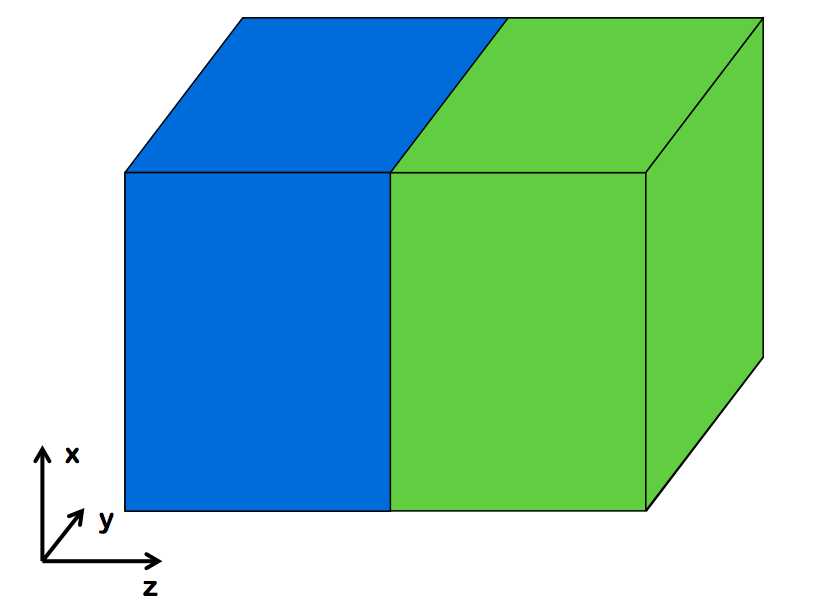
\includegraphics[scale=0.25]{AABB.png}
		\caption{Binary--mixture periodic in all dimensions}
		\label{AABB}
	\end{subfigure}
	\begin{subfigure}{.5\linewidth}
		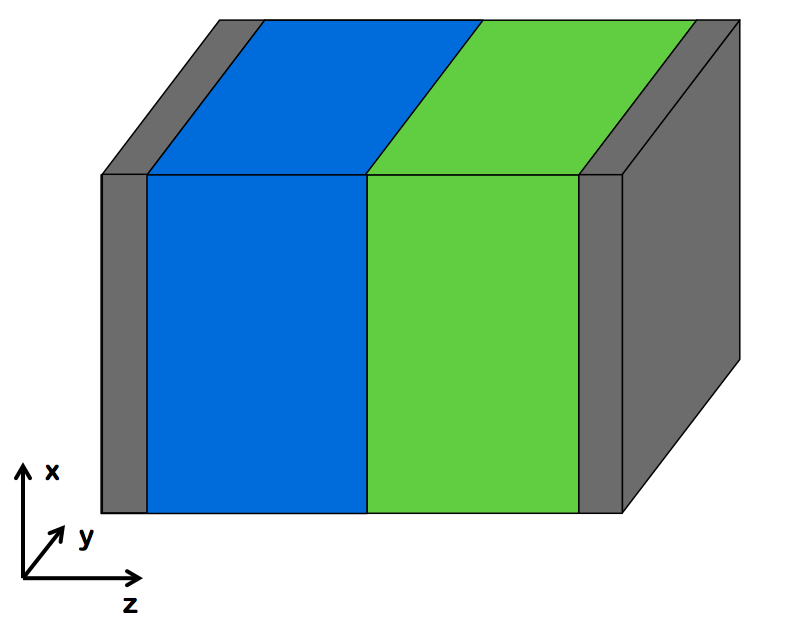
\includegraphics[scale=0.25]{AABB_piston.png}
		\caption{Binary--mixture confined by planar walls} 
		\label{AABB_piston}
	\end{subfigure}
	\caption{Both the systems studied incorporated a partially miscible binary--mixture of Fluid A (blue) and Fluid B (green).
For the mixture periodic in all dimensions, the pressure is regulated using a Nos\'{e}--Hoover barostat.
In the confined fluid, the walls are used to create a piston and an external force equal to $P_{\mathrm{ext}} \times A_{\mathrm{wall}}$ is applied.
}
	\label{SetUp}
\end{figure}

\subsection{Interaction Model}\label{InteractionModel}
The fluids were modelled using spherical particles and their interaction was tuned to a pair--wise truncated Lennard--Jones potential:
\begin{equation}
V \left( \mathbf{r}^{\mathrm{N}} \right) = \frac{1}{2} \sum_{i\neq j} \phi \left( r_{ij} \right)
\end{equation}
where
\begin{align}
\label{LJ}
\phi \left( r_{ij} \right) &= 4 \epsilon_{ij} \left( \left( \frac{\sigma_{ij}}{r_{ij}}\right)^{12} - \left( \frac{\sigma_{ij}}{r_{ij}}\right)^{6} \right)\ \mathrm{for}\ r \leq r_{c}\\
\phi \left( r_{ij} \right) &= 0\ \mathrm{for} r > r_{c}.
\end{align}
This potential involves an attractive $r_{ij}^{-6}$ term accounting for the long--range Van der Waal's interaction and a short--range $r_{ij}^{-12}$ repulsive term corresponding to the Pauli repulsion between particles.
The length--scale of the potential is given by $\sigma_{ij}$ (chosen to be equal for all pairs of $i$ and $j$) whilst the parameter $\epsilon_{ij}$ determines the strength of the interaction. 

The miscibility of the two fluids (A and B) can be controlled using the relative values of the interaction parameter; in this study the values chosen were:
\begin{align}
\epsilon_{A,A} &= \epsilon_{B,B} = 1.0,\\
\epsilon_{A,B} &= 0.55,
\end{align}
in agreement with previous studies on similar Lennard--Jones binary--mixtures.\cite{MorenzoRazo,Blas,HolgerBoppHampe}
The cutoff for the potential was chosen to be $r_{c} = 4\ \sigma$.

\subsection{Reduced Units}\label{ReducedUnits}
Physical quantities including distances and energies are expressed in terms of reduced units.
For a Lennard--Jones system, the basic units are $\sigma$ for length, $\epsilon$ for energy and $m$ for mass, from which all other units may be derived.\cite{FrenkelSmit}
Physical quantities become dimensionless when expressed in terms of these units, for example $r^{*} \equiv r / \sigma$.
Scaled coordinates expressed relative to the simulation box size are also used, for example $z' = z^{*} / L_{z^{*}}$ where $L_{z^{*}}$ is the dimension of the box in the z--direction.
These are useful if the box--dimensions vary, such as when a barostat acts on the system.

\subsection{Thermostats}\label{Thermostats}
In molecular dynamics simulations, the temperature is controlled using thermostats, which simulate the coupling of the system to an external heat bath.

Thermostats work by applying a stochastic frictional force to particles, either by adding a random force to momenta (Langevin)\cite{Langevin} or reassigning the velocity of randomly chosen particles to that obtained from the Maxwell distribution (Anderson)\cite{AndersonTherm}.
The Nos\'{e}--Hoover thermostat was used throughout this study.
This introduces a fictitious frictional force into the equations of motion which adjusts the particle velocities until the temperature is equal to the desired value.\cite{NoseHoover1, NoseHoover2, NoseHoover3}
The equations of motion in 3D become:
\begin{align}
m_{i}\frac{\mathrm{d}^{2}\mathbf{r}_{}}{\mathrm{d} t ^{2}} =& \mathbf{f}_{i} - \zeta m_{i} \mathbf{v}_{i}\\
\frac{\mathrm{d} \zeta (t)}{\mathrm{d} t} =& \frac{1}{Q}\left[ \sum_{i=1}^{N} m_{i} \frac{\mathbf{v}^{2}_{i}}{2} - \frac{3N+1}{2}k_{\mathrm{B}}T\right].
\end{align}
The result is a system where the energy fluctuates but the combined energy of the system and heat bath remains constant, maintaining a canonical ensemble.

\subsection{Barostats}\label{Barostats}
The bulk pressure of the fluid must also be held constant.
A piston provides the simplest method and is relatively easy to create; the fluid is confined between two solid walls and a force equal to $P_{ext} \times A_{wall}$ is applied.
This was used for studying the binary--mixture confined between two walls.
In the case of Marangoni flows, a thermocapillary effect will also occur at the boundary of the liquid and the solid piston.
The interface must be sufficiently far from the walls such that this thermocapillary force can be ignored.
Only the interfacial force should then be applied in the final simulation.

Alternatively a Nos\'{e}--Hoover barostat can regulate the pressure by adjusting the simulation box dimensions and altering the equations of motion accordingly. \cite{NoseHoover1, NoseHoover2, NoseHoover3}
When studying surface effects, the box size must only be changed in the direction perpendicular to the interface, since any other direction will alter its area and create an error in the thermodynamic pressure,
\begin{equation}
P = - \left( \frac{\partial F}{\partial V} \right)_{T} + \gamma \left( \frac{\partial A}{\partial V} \right)_{T}.
\end{equation}

\subsection{Preparing the system}\label{SystemPrep}
The fluid was prepared from a face--centred cubic lattice with a spacing of $1.64414\ \sigma$ and a simulation box size of $L_{x^{*}}=13.1531$, $L_{y^{*}}=13.1531$ and $L_{z^{*}}=32.8828$.
This lattice was melted over $2\times 10^{6}$ timesteps of length $0.001\ \tau$ to generate a fluid state.
The barostat was set to a pressure of $P^{*} = 0.1$ and the temperatures used were $T^{*} = 0.8$ and $T^{*} = 0.9$, ensuring the system occupied the liquid region of the Lennard--Jones phase space.\cite{Smit}
Solid walls in the system were constructed with a harmonically bonded lattice using a spring constant of $K^{*} = 2500$ and an equilibrium bond length of $r^{*}_{0}=1.163$.

\subsection{Calculating the stress tensor}\label{CalcStress}
The Virial stress tensor was calculated using an in--built function within the LAMMPS package, which returns the stress tensor for each atom.
However, LAMMPS does not have a method for calculating the Irving--Kirkwood stresstensor.
Instead this was calculated by dumping the particle positions on a given timestep to a file and post--processing.
The stress tensor was then computed using a programme written by R. Ganti and adapted for the specific systems studied.
Since the Virial method is implemented in parallel whilst the Irving--Kirkwood method is not, the Irving--Kirkwood stress was significantly more expensive to compute, incurring approximately a 4-fold increase in computational time.

\subsection{Computing averages}\label{ComputeAve}
Usually time--averages of physical observables are calculated in molecular dynamics simulations. 
In the systems studied, the observables are the number density, stress tensor and particle velocities.
Their values were measured every timestep and spatially averaged for $400$ planar slabs across the z--dimension of the box.
These spatial averages were then time--averaged over the full duration of the simulation.

Under the ergodic hypothesis, time--averages can be equated to ensemble averages for an infinitely long simulation time.\cite{Bopp2008}
Practically, however, these averages must be evaluated over a finite time period and have an associated statistical error.
The method of block--averaging, developed by Flybjerg and Peterson, provides an efficient technique for computing this error.\cite{Flyvbjerg1989}
They show that the variance of an observable, $A$, can be estimated by
\begin{equation}
\mathrm{var}(A) \geq \left< \frac{C_{0}}{n-1} \right>,
\end{equation}
where $C_{0}$ is the value of the time-correlation function for the block--transformed data at $t=0$ and is given by
\begin{equation}
C_{0} \equiv \frac{1}{n} \sum_{k=1}^{n} \left( A_{k} - \bar{A} \right) \left(A_{k} - \bar{A} \right).
\end{equation}
A lower bound for the variance can be calculated by finding the block length at which this estimate reaches a plateau.
Furthermore, the error in the variance can be estimated as 
\begin{equation}
\sqrt{\frac{2}{n-1} \times \frac{C_{0}}{n-1}}.
\end{equation}

\begin{figure*}[h]
\hspace{-3em}
	\begin{subfigure}{.5\linewidth}
                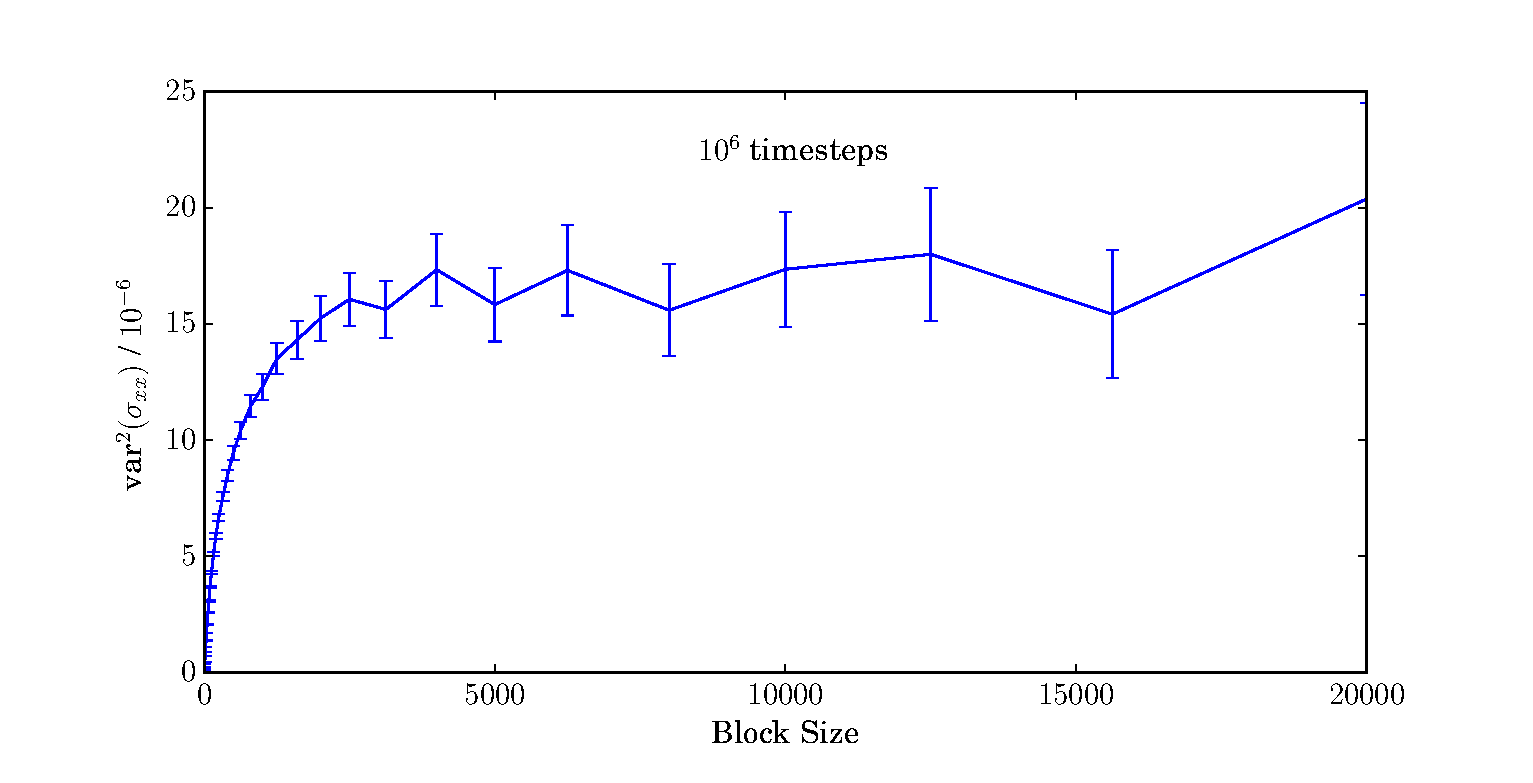
\includegraphics[scale=0.6]{block_average_1e6.eps}
                \caption{Simulation time = $1000\ \tau$}
        \end{subfigure}
\hspace{2em}
        \begin{subfigure}{.5\linewidth}
                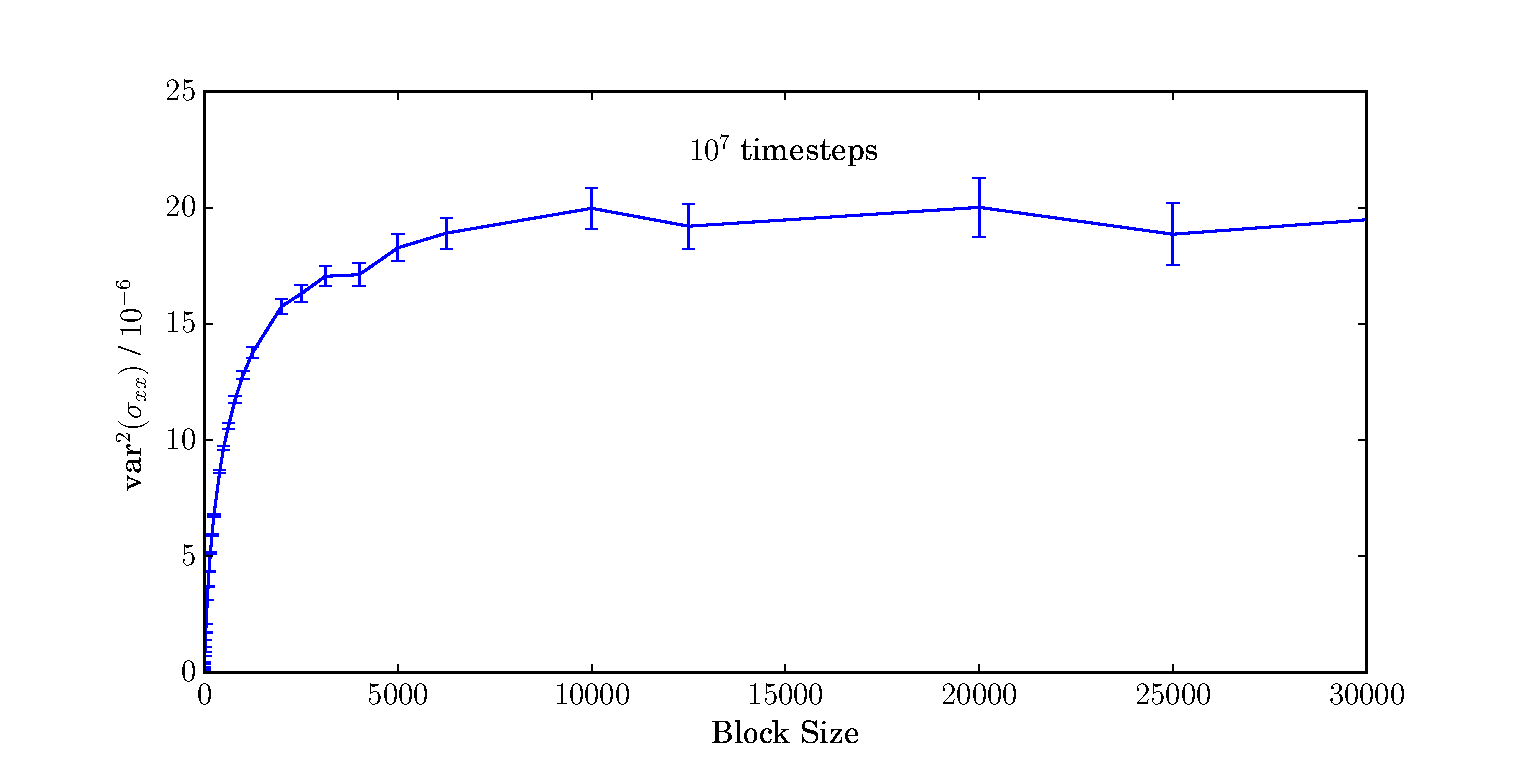
\includegraphics[scale=0.6]{block_average_10e6.eps}
                \caption{Simulation time = $10000\ \tau$}
	\end{subfigure}
	\caption{The blocking analysis for a system identical to those studied is compared for simulation times of $1000\ \tau$ and $10000\ \tau$.
Plateaus in the estimate of the variance begin at block lengths of approximately $5\ \tau$ and $10\ \tau$ respectively.
The error in the variance does not become significant until much larger block lengths.
Throughout the subsequent simulations, a block size of $10\ \tau$ was used.
This ensured decorrelation of the data and produced a reliable estimate of the statistical error.
}
\label{blocking}
\end{figure*}

A blocking--analysis for a binary--mixture identical to those used throughout this study was executed over a simulation time of $1,000\ \tau$ and $10,000\ \tau$, as shown in Figure \ref{blocking}.
The plateau begins at a block length of $10\ \tau$ for the long simulation and $5\ \tau$ for the shorter run, with little increase in the error of the variance until a much larger block size.
Considering this result, a block length of $10\ \tau$ was used to provide a good estimate for the error of all time--averages calculated in the subsequent simulations.
\FloatBarrier

\subsection{Modelling surfactant molecules}\label{ModellingSurfactants}
\begin{figure*}[h]
\centering
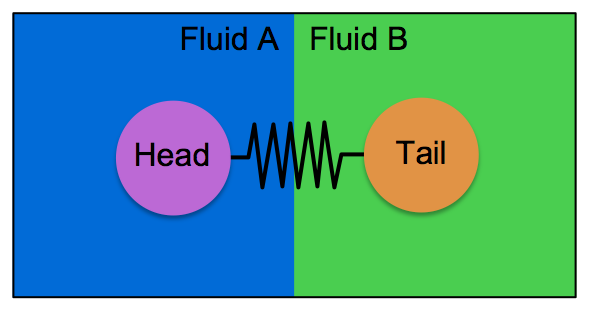
\includegraphics[scale=0.4]{surfactant.png}
\caption{Surfactant molecules are represented by a pair of spherical Lennard--Jones particles connected by a harmonic bond. 
The head particle has a stronger interaction with Fluid A ($\epsilon_{H, A} = 1.33$ and $\epsilon_{H, B} = 0.17$) whilst the tail has a stronger interaction with Fluid B ($\epsilon_{T, A} = 0.17$ and $\epsilon_{T, B} = 1.33$).
This generates the desired surface active behaviour.
 }
\label{surfactant}
\end{figure*}
To investigate the effects of surfactants on the Marangoni effect, the surfactant molecules were modelled as a pair of Lennard--Jones particles connected by a harmonic bond with spring constant $K^{*} = 25$ and equilibrium bond length $r^{*}_{0}=1.63$.
Inspired by Howes and Radke's study on non--ionic surfactants,\cite{HowesSurfactant} the `head' particle has a stronger interaction with Fluid A particles, ($\epsilon_{H, A} = 1.33$ and $\epsilon_{H, B} = 0.17$) whilst the `tail' particle has a stronger interaction with Fluid B particles ($\epsilon_{T, A} = 0.17$ and $\epsilon_{T, B} = 1.33$).
The `head' and `tail' groups interact with each other with strength $\epsilon_{H, T} = 1.00$.
\FloatBarrier

\subsection{Software details}\label{SoftwareDetails}
All molecular dynamics simulations were carried out using the LAMMPS (Large Atomic and Molecular Massively Parallel Simulator) package.\cite{LAMMPS}
Additional processing was carried out using Numpy.\cite{NumPy}
All graphical figures were plotted using Matplotlib.\cite{MatPlotLib}





\newpage
\addcontentsline{toc}{chapter}{Bibliography}
\bibliography{thesis}
%\thispagestyle{empty}
\newpage
\cleardoublepage

\end{document}
